\documentclass[11pt]{article}
\usepackage[margin=1in]{geometry}
\usepackage[T1]{fontenc}
\usepackage{lmodern}
\usepackage{amsmath,amssymb,amsthm,bm,mathtools}
\usepackage{graphicx,booktabs,array,microtype,xcolor}
\usepackage{hyperref}
\emergencystretch=3em
\raggedbottom
\hypersetup{colorlinks=true,linkcolor=blue!45!black,citecolor=blue!45!black,urlcolor=blue!45!black,pdftitle={Initial-state matching and stability diagnostics for a counter-streaming electron-fluid closure},pdfauthor={Taylor Kalin}}
\newcommand{\R}{\mathbb R}
\newcommand{\E}[1]{\mathbb E\!\left[#1\right]}
\newcommand{\norm}[1]{\left\lVert #1\right\rVert}
\newcommand{\dd}{\mathrm d}
\DeclareMathOperator{\tr}{tr}
\DeclareMathOperator{\diag}{diag}
\newtheorem{proposition}{Proposition}[section]
\newtheorem{lemma}[proposition]{Lemma}
\newtheorem{corollary}[proposition]{Corollary}
\title{Initial-state matching and stability diagnostics for a counter-streaming electron-fluid closure}
\author{\textbf{Taylor Kalin}\\[3pt]
\small\href{https://taylorkalin.com}{taylorkalin.com}\quad
\href{mailto:teylersf@gmail.com}{teylersf@gmail.com}\\
\small ORCID: \href{https://orcid.org/0009-0003-9000-9315}{0009-0003-9000-9315}}
\date{28 October 2026}
\begin{document}
\maketitle
\begin{abstract}
We examine the initial-state matching and closure interpretation in
arXiv:2607.07106v1 using its published input decks, archived initial moments,
and explicit continuum tests. The central two-population pressure and
third-moment identities are correct. However, the PIC input specifies a
proper-momentum drift where the fluid input specifies ordinary velocity.
In the two archived cells straddling the lower current-sheet center, the
density-weighted initial PIC moment current differs by about 11.5\% from
the magnetostatic current implied by the staggered magnetic curl. Its
Cartesian thermal pressures are about 20\% below the fluid initialization in
$p_{xx}$ and 38.4\% below in $p_{zz}$.
A matched-state rerun
is needed to determine the effect on the nonlinear comparison. Separately,
the stated finite-isotropization closure has an overstable longitudinal
mode with growth about $0.00952\omega_{pe}$ in a homogeneous two-Maxwellian
equilibrium certified as stable to collisionless longitudinal electrostatic
perturbations by the Penrose criterion.
We give the linear system, constraint checks, a correction to the
symmetry-plane density argument, and a relative heat-flux error bound
that accounts for imbalance and cancellation. The calculations distinguish
valid mixture algebra, empirical benchmark evidence, and claims requiring
additional validation. No new PIC or Gkeyll reconnection simulation is claimed.
\end{abstract}
\section{Introduction and scope}
\label{sec:introduction}
Counter-streaming electron populations provide a useful representation of the
strongly non-Maxwellian distributions generated during collisionless magnetic
reconnection. McGrae-Menge and collaborators~\cite{original} report that tagging
electrons by their initial side of a current sheet isolates sub-populations
whose intrinsic third moments are small compared with their combined heat
flux. Their exact moment decomposition explains how relative motion and
population asymmetry can generate a substantial aggregate third moment even
when each population has little intrinsic heat flux. Evolving additional
population moments is therefore physically motivated.

The present study examines two separate questions that this useful mechanism
does not settle: whether the numerical comparison starts from matched physical
states, and whether the implemented finite-relaxation closure has the kinetic
stability properties attributed to it. These are testable questions about
the identified source version and model, rather than an assertion that the
underlying mixture interpretation is wrong.

Our first result uses the authors' publicly archived initial moments and input
decks~\cite{dataset}. Identical nominal drift expressions enter a proper-momentum
initializer in PIC and an ordinary-velocity initializer in the fluid model.
The recorded initial moments show a current and pressure mismatch consistent
with that distinction. This is a reproducible control issue for interpreting
the nonlinear comparison; its eventual dynamical effect cannot be determined
from initial-state analysis alone.

Our second result is a controlled longitudinal stability test of the stated
continuum isotropization closure. A positive two-Maxwellian equilibrium is
stable to longitudinal electrostatic perturbations under the established
Penrose criterion~\cite{penrose1960}, but its
finite-relaxation fluid counterpart has an overstable mode. We give an explicit
linear system and check both its eigenvalue residual and Gauss constraint.
The test is homogeneous and nonrelativistic. It does not replace the source's
inhomogeneous reconnection calculation or show that the identified mode caused
any of its plotted features.

Two further results make the interpretation more precise. Continuity depends
on the divergence of the mass flux, so a zero normal velocity at a symmetry
plane does not prohibit density accumulation there. A conditioned third-moment
error bound also shows why a thermal-to-drift speed ratio alone does not give
a universal relative-error guarantee when population contributions cancel.
Neither result disputes the empirical parameter trend in the published scan.

\subsection{Relation to established work}
Heat-flux closure and its effect on collisionless response are established
subjects. Hammett and Perkins~\cite{hammett1990} developed fluid moment models
for Landau damping, while Wang and collaborators~\cite{wang2015} compared
multifluid moment models with PIC reconnection. Goldman and
collaborators~\cite{goldman2020} studied multibeam energy moments and the
distinction between component and aggregate centering. The mixture algebra
used below belongs to this established moment framework.

Closure-dependent instability spectra are also known. Ng and
collaborators~\cite{ng2019} demonstrate why a pressure-tensor model must be
checked against kinetic response rather than judged solely by its retained
variables. Our finite-relaxation example supplies a concrete test associated
with the closure and reference rate in the present source; we do not claim the
general phenomenon of closure-dependent unstable modes as new.

Work on heat-flux closure for nonlinear electrostatic two-stream systems
\cite{ingelsten2025,ingelsten2026} further limits a literal reading of broad
claims that no fluid closure can capture non-Maxwellian counter-streaming.
It does not establish prior use of the specific tagged-population closure in
electron-only reconnection. Our analysis therefore addresses explicit
initialization, continuity and stability statements, and preserves the
source's application-specific empirical evidence.

\subsection{Audited version and available evidence}
The supplied ten-page PDF is byte-identical to a fresh versioned download of
arXiv:2607.07106v1: 7,847,791 bytes, SHA-256
\texttt{fc5344e2ba8f4db98baf90d805bb6b7ce}\\
\texttt{8835c32ea7bf54bba4d62f405b955a3}.
The official history checked on 28 October 2026 lists the 8 July v1 and no
later revision or journal reference. The PDF displays 9 July, while the
experimental HTML displays a different compilation date. The original TeX
uses \verb|\date{\today}|; those compilation dates do not identify additional
scientific revisions. Appendix~\ref{app:source-evidence} records source and
data locators. No original author has been contacted, and no author
confirmation or private simulation-build access is claimed.

\section{Initial-state matching in the supplied input decks}
\label{sec:initialization}

The source compares a relativistic PIC calculation with nonrelativistic
ten-moment fluid calculations and describes their common initialization in
Appendices A and C~\cite{original}. The deposited reference-case decks and
initial moments make the physical matching of those states directly
testable~\cite{dataset}. Equal numerical drift and temperature parameters
need not specify equal laboratory-frame velocity moments in the two codes.
This issue concerns the controlled comparison; the mixture identities do
not depend on either code's initialization convention.

\subsection{A proper-momentum parameter is used as a fluid velocity}
The PIC deck sets \texttt{use\_spatial\_ufl=.true.} and supplies the curl-derived
drift expressions as \texttt{spatial\_ufl}. The official OSIRIS reference
defines these inputs as proper velocities, or momentum divided by particle
mass, with relativistic boosting as the default~\cite{osirisudist}.
No classical-addition override appears in the posted deck. The Lua decks
instead set nonrelativistic conserved momentum density to $\rho\mathbf v$
using the same expressions. This is the ordinary velocity variable of the
ten-moment equations~\cite{wang2015}.

Writing $\mathbf U=\mathbf p/(m_ec)$, a cold population with proper drift
$\mathbf U$ has
\begin{equation}
 \frac{\mathbf v}{c}=\frac{\mathbf U}{\sqrt{1+|\mathbf U|^2}}.
 \label{eq:proper-ordinary}
\end{equation}
Thus the same numerical vector used for $\mathbf U$ in PIC and $\mathbf v/c$
in the fluid initializer does not match the physical cold drift. At the
unperturbed lower sheet center, the reference expressions give approximately
$(0,0,0.5)$: the cold PIC speed is $0.4472136c$, whereas the prescribed fluid
speed is $0.5c$. The fractional difference is $10.56\%$. It persists when
the thermal spread tends to zero at fixed $B_{\mathrm{Reconn.}}=0.5$ and sheet
width $d_e$; low thermal beta alone does not remove it. Equation
\eqref{eq:proper-ordinary} is a cold-limit explanation. A finite-temperature
mean must be measured after loading rather than identified with that limit.

\subsection{A conditional finite-temperature loading calculation}
The complete 155-line posted PIC deck contains two thermal-distribution
blocks with $\sigma=0.111803$, and no classical-addition override or include
directive. The inspected public OSIRIS loader draws independent Gaussian
thermal proper-momentum components and boosts each particle without changing
its weight~\cite{osirisloader}. With $c=1$, for thermal momentum
$\mathbf w\sim\mathcal N(0,\sigma^2I)$ and proper drift $\mathbf U$, this rule is
\[
 \gamma_0=\sqrt{1+|\mathbf w|^2},\quad G=\sqrt{1+|\mathbf U|^2},\quad
 \mathbf p=\mathbf w+\mathbf U
 \left(\gamma_0+\frac{\mathbf w\cdot\mathbf U}{G+1}\right),\quad
 \mathbf v=\frac{\mathbf p}{G\gamma_0+\mathbf w\cdot\mathbf U}.
\]
This is a prediction conditional on the public loading rule, not an
identification of the original executable. With $\beta=|\mathbf U|/G$ and
$z=w_\parallel/\gamma_0$, pairing opposite Gaussian momenta gives
\[
 \mathbb E[v_\parallel]
 =\beta\left[1-(1-\beta^2)
 \mathbb E\left(\frac{z^2}{1-\beta^2z^2}\right)\right]<\beta
\]
for positive drift and nonzero thermal spread. Thus the mean can fall below
the cold conversion without an additional force. An invariant scalar
distribution sampled at equal laboratory time would require a different
Jacobian-weighted measure; it must not be silently substituted for this
unweighted sample-boost rule.

At $\mathbf U=(0,0,0.5)$ the finite-temperature mean is $0.44297014c$,
below the cold $0.44721360c$. Evaluating the full spatial drift expressions
and perturbations at the two lower diagnostic rows gives an $x$-averaged
zero-shape prediction $0.44197416c$. A separate, unfitted sensitivity uses
the declared quadratic interpolation, the recorded moment-cell offset and
the posted $25\times25$ regular particle lattice. Summing the standard
quadratic weights over their support gives the following conditional values:
\begin{center}
\begin{tabular}{lrr}
\toprule
Quantity & $Y=15.95d_e$ & $Y=16.05d_e$ \\
\midrule
Archived $\overline v_z/c$ & 0.44098722 & 0.44087669 \\
Pointwise loading prediction & 0.44197416 & 0.44197416 \\
Quadratic-shape prediction & 0.44098868 & 0.44098868 \\
Archived $P_{xx}$ & 0.00994868 & 0.00997543 \\
Quadratic-shape $P_{xx}$ & 0.00996490 & 0.00996490 \\
Archived $P_{zz}$ & 0.00769653 & 0.00769303 \\
Quadratic-shape $P_{zz}$ & 0.00770632 & 0.00770632 \\
\bottomrule
\end{tabular}
\end{center}
These pressure predictions use expected raw moments centered at each node
before averaging, in the infinite-particle limit. No temperature, drift,
shape width or perturbation is fitted to the archived values. Quadrature
orders 12, 20, 32 and 48 agree in the quadratic mean to about
$5\times10^{-16}c$; an independent Cartesian quadrature checks the reduced
moment calculation to $1.73\times10^{-15}$ in the tested quantities.
This is a conditional consistency check of the scale of the additional
reduction below the cold value. Agreement does not identify the historical
loader or the custom diagnostic kernel.
The standard public deposition kernel is not verified as the original
custom velocity diagnostic's kernel, so the pointwise prediction and shape
sensitivity remain distinct. Neither is a new PIC run or a confidence
statement about the unidentified original build.

\subsection{Archived initial current and staggered magnetic curl}
The original data authors explicitly define the archived diagnostic
\texttt{vfl\_i} as $(1/n)\int f v_i\,\dd^3v$~\cite{dataset}.
It is therefore an ordinary mean velocity, even though the input parameter
\texttt{ufl} is a proper-momentum parameter. With the source normalization
$q_e=-1$, the physical moment current is
\begin{equation}
 J_z^{\mathrm{mom}}=-\left(n_1\overline v_{1z}+n_2\overline v_{2z}\right).
 \label{eq:archived-moment-current}
\end{equation}
The selected initial density diagnostics give $n_1+n_2=1$ to within
$1.5\times10^{-8}$. No particle tracking or new time integration is needed
to evaluate this current.

The HDF5 files also record their grid offsets: density and velocity moments
have $(0.5,0.5)$, $B_x$ has $(0.5,1)$ and $B_y$ has $(1,0.5)$.
The backward staggered differences therefore place
\begin{equation}
 J_{z,i,j}^{B}=
 \frac{B_{y,i,j}-B_{y,i-1,j}}{\Delta x}
 -\frac{B_{x,i,j}-B_{x,i,j-1}}{\Delta y},\qquad
 \Delta x=\Delta y=0.1d_e,
 \label{eq:archived-magnetic-curl}
\end{equation}
on the moment-cell centers. Periodic differencing makes the first term's
$x$ average exactly zero. The raw data use $y\in[-32,32]d_e$; the paper's
coordinate is $Y=y+32d_e$, so its lower sheet is at $Y=16d_e$.

\begin{table}[htbp]
\centering
\caption{Initial $x$-averaged currents in the cells adjoining the lower sheet.
The deficit is $1-\langle J_z^{\mathrm{mom}}\rangle_x/
\langle J_z^B\rangle_x$. Currents use the source's normalized units.}
\label{tab:initial-current}
\begin{tabular}{rrrr}
\toprule
$Y/d_e$ & $\langle J_z^{\mathrm{mom}}\rangle_x$ &
$\langle J_z^B\rangle_x$ & Deficit \\
\midrule
15.95 & $-0.44098723$ & $-0.49833998$ & $11.5088\%$ \\
16.05 & $-0.44087669$ & $-0.49833998$ & $11.5309\%$ \\
\bottomrule
\end{tabular}
\end{table}

The supplied fluid initializer prescribes an $x$-averaged ordinary velocity
$0.49875256c$ in these same cells. The archived PIC means are
$0.44098722c$ and $0.44087669c$, approximately $11.6\%$ smaller. The small
difference between this continuum prescription and Table~\ref{tab:initial-current}'s
staggered curl does not explain the observed deficit. The adjacent cells at
the other sheet show the same effect with reversed current sign.

The result is not restricted to these four illustrative cells.
Across all 640 rows, the relative $\ell^2$ discrepancy between the
$x$-averaged moment-current and Yee-curl profiles is $9.8265\%$.
Restricting to $14\leq Y/d_e\leq18$ or $46\leq Y/d_e\leq50$ gives
$9.8287\%$ and $9.8408\%$, respectively. These are norms of the
one-dimensional averaged profiles, not norms of the full two-dimensional
fields. Figure~\ref{fig:full-profile} displays both sheets and the full domain.
The input-prescribed current differs from the Yee profile by only $0.0630\%$
in the full-profile relative norm.

As a deterministic discretization sensitivity, averaging the staggered fields
onto cell centers before a centered derivative changes the curl profile by
$0.3755\%$ in that norm. This is a deliberately smoothed representation,
not an alternative reading of the recorded Yee offsets. The central-cell
moment-current deficits remain about $11.05$--$11.10\%$ against that smoothed
profile. Eight contiguous 60-column blocks at $Y=15.95d_e$ have moment-current
means between $-0.4417104$ and $-0.4404351$, compared with the Yee mean
$-0.4983400$. The per-column standard deviation is $0.0019906$.
These spatial summaries are descriptive; correlated particle deposition and
the imposed perturbation preclude treating them as independent-sample
confidence intervals.

Here $J_z^{\mathrm{mom}}$ is a moment-based physical diagnostic. We have not
reloaded OSIRIS's native charge-conserving deposited current, which can differ
from a simple $qv$ deposition. These numbers therefore do not specify the
exact discrete electric-field update of the original executable.
In the normalized continuum equations,
$\partial_t E_z=(\nabla\times\mathbf B)_z-J_z$.
The comparison is a continuum magnetostatic diagnostic. It does not establish
an initial transient in the native numerical electric-field update.

\subsection{The laboratory-frame pressure moments also differ}
The record defines its second-moment diagnostics without a density
normalization: $M_{s,ii}=\int f_s v_i^2\,\dd^3v$~\cite{dataset}.
Following the source's own pressure definition, at $m_e=1$ we compute
\begin{equation}
 P_{ii}=M_{1,ii}+M_{2,ii}-n\overline v_i^2.
 \label{eq:archived-pressure}
\end{equation}
The posted fluid initializers prescribe an isotropic thermal pressure
\[
p_{\mathrm{fl}}=n_0(0.111803)^2=0.012499910809.
\]
The archived initial fluid \texttt{.bp} fields independently confirm this
pressure in both fluid models, as detailed below. The measured ratios to
the archived fluid pressure are
\begin{center}
\begin{tabular}{rrr}
\toprule
$Y/d_e$ & $\langle P_{xx}\rangle_x/p_{\mathrm{fl}}$ &
$\langle P_{zz}\rangle_x/p_{\mathrm{fl}}$ \\
\midrule
15.95 & 0.795900 & 0.615727 \\
16.05 & 0.798040 & 0.615447 \\
\bottomrule
\end{tabular}
\end{center}
For example, at $Y=15.95d_e$ the archived values are
$\langle P_{xx}\rangle_x=0.00994868$ and
$\langle P_{zz}\rangle_x=0.00769653$. The latter is about $38.4\%$ below
the archived fluid pressure. These are the ordinary-velocity covariance
moments defined in the source, not components of a relativistic
energy--momentum tensor. A common rest-frame thermal-momentum parameter
does not imply equal laboratory-frame velocity covariance after a boost.
Centering the pressure after averaging in $x$ instead adds the
density-weighted variance of the resolved mean flow. At the four central
rows this changes either diagonal component by approximately
$4\times10^{-6}$, far smaller than the reported pressure mismatch;
the source definition and our principal result center each cell first.
Figure~\ref{fig:initial-state} shows the local $x$-averaged profiles.

\subsection{Corroboration against the saved fluid state}
We reloaded five initial BP snapshots: the one-fluid electron state, both
two-fluid electron states, and each model's electromagnetic field. They
record time and frame zero, a single available step, the same
$480\times640$ grid and bounds, zero ghost cells and polynomial order zero.
Each file's embedded base64 input deck decodes byte-for-byte to the posted
Lua file. This checks the input used in the saved output, rather than assuming
that the separate prescription was executed unchanged.

The ten stored components are $\rho$, the three $\rho u_i$, and the six
symmetric raw second moments. Their order independently matches the official
Gkeyll conservative-variable layout~\cite{gkeylllayout} and is checked against every returned
initializer component over all 307,200 cells, including off-diagonal moments
and the field components. The largest one-fluid component error is
$4.38\times10^{-16}$; the summed two-fluid state differs from the one-fluid
state by at most $1.12\times10^{-16}$. Aggregate pressure is reconstructed
after summing the conservative population moments. Thus the earlier
comparison with the prescribed initial state is corroborated by the actual
archived state.

Against either reloaded fluid model, the full 640-row, $x$-averaged PIC
profiles have relative $\ell^2$ differences of $9.8675\%$ for $J_z$,
$8.3169\%$ for $P_{xx}$ and $9.5440\%$ for $P_{zz}$. At the two lower central
rows the actual fluid current is $-0.4987525573$, giving moment-current
deficits $11.5820\%$ and $11.6041\%$. The local pressure ratios reported
above are unchanged. These comparisons concern physical velocity moments,
not native PIC current deposition or later-time dynamics.

All selected PIC files have \texttt{TIME=0} and \texttt{ITER=0}; the fluid
files have time and frame zero. No explicit time-averaging attribute appears.
This verifies the posted snapshot metadata, not the impossibility of an
undocumented operation in the unidentified PIC build. A complete inventory
of all 223 PIC ZIP entries, including 94 scientific files, identifies no
native deposited-current diagnostic. We therefore cannot make the requested
native-current comparison from this deposit and do not substitute the
\texttt{UDIST} moment current for it.

\subsection{What a controlled comparison requires}
The data establish an initial-state mismatch in the posted comparison. They
do not establish how much of any later reconnection difference it causes.
That requires reruns with controlled initial moments and numerical refinement.
One constructive test is to initialize the fluid models from the measured
PIC $n$, $\overline{\mathbf v}$ and $P_{ij}$, preserving the intended population
labels. Another is to calibrate the PIC loading to a prescribed physical
fluid state and then verify the deposited moments. The cold conversion in
Eq.~\eqref{eq:proper-ordinary} is necessary for a cold drift match, but by
itself does not guarantee a finite-temperature pressure or current match.

The fluid BP metadata records Gkeyll changeset \texttt{9663ea594e80+}; its
plus suffix does not identify a clean exact source tree or executable.
The original PIC executable remains unidentified. The current public OSIRIS
code inspected for documentation does not expose the
authors' custom \texttt{vfl}/third-moment diagnostic implementation.
Our diagnostic interpretation follows their explicit dataset definitions
and file metadata. The selected files in this section are initial snapshots.
Their archived-data reanalysis is distinct from the new clean-source fluid
evolutions in Section~\ref{sec:controls}; it supplies no causal attribution
of the source's later nonlinear results by itself.

\begin{figure}[tbp]
\centering
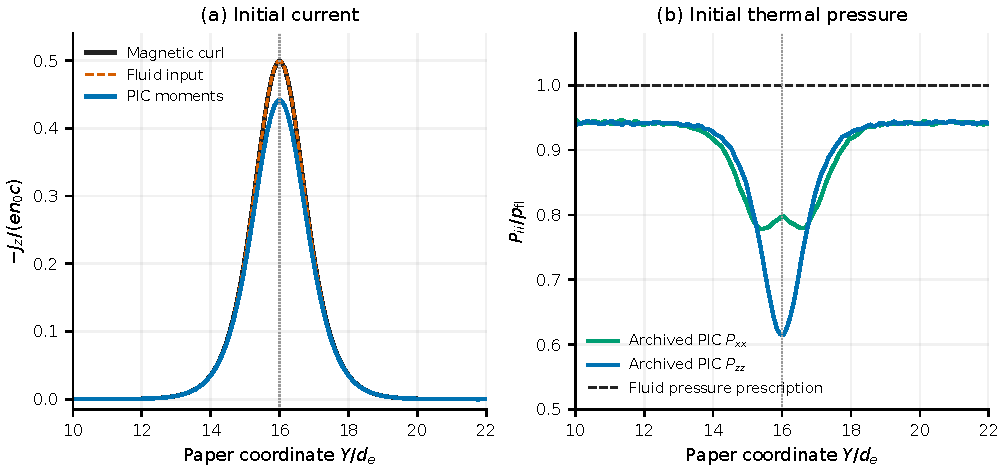
\includegraphics[width=\linewidth]{../figures/initial-state.pdf}
\caption{Reanalysis of the archived initial state near the lower sheet.
Left: the ordinary-velocity moment current differs from both the staggered
magnetic curl and the posted fluid prescription. Right: the local centered
pressure components, averaged in $x$ after centering, differ from the isotropic
fluid pressure. The profiles use the authors' archived diagnostics and
their published definitions~\cite{dataset}. The drawn fluid curves use the
initializer; the reloaded initial fluid output independently corroborates
them to roundoff. No new simulation is shown.}
\label{fig:initial-state}
\end{figure}

\begin{figure}[tbp]
\centering
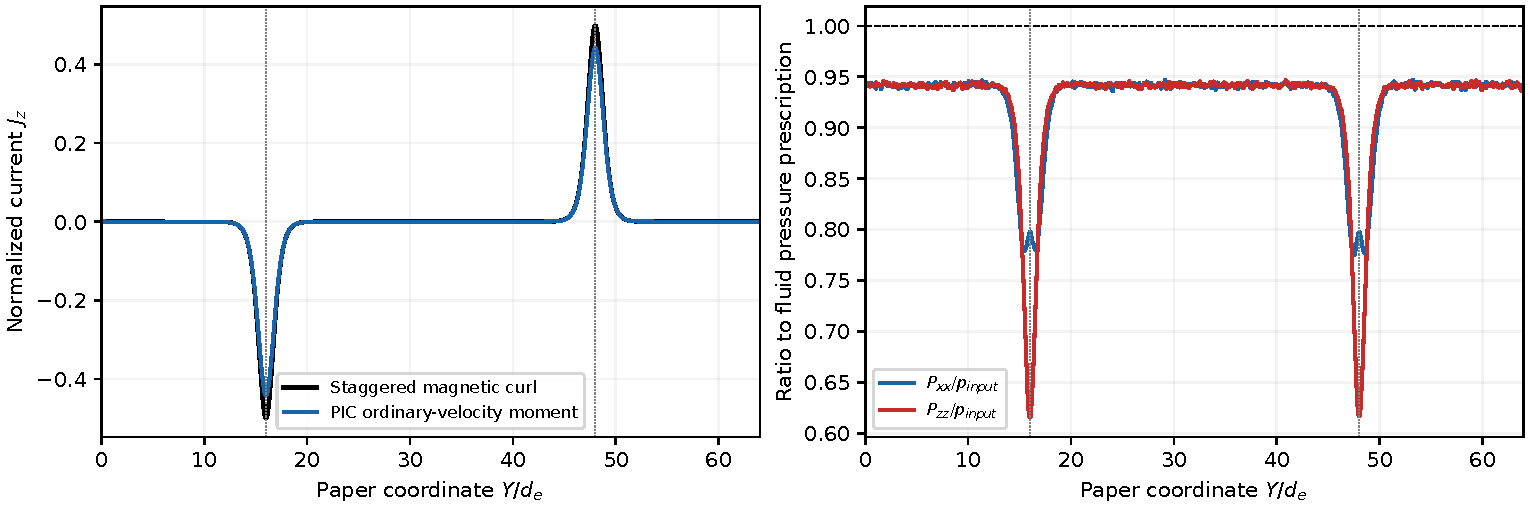
\includegraphics[width=\linewidth]{../figures/profile-sensitivity.pdf}
\caption{Full-domain, $x$-averaged archived PIC profiles at $t=0$, with both
current sheets visible. Left: physical moment current and the correctly
staggered magnetic curl. Right: velocity-covariance pressures divided by
the fluid pressure confirmed in the archived output. The figure extends the local view; it is neither
an independent simulation nor a native deposited-current diagnostic.}
\label{fig:full-profile}
\end{figure}

\section{A controlled linear-stability test}
\label{sec:stability}
The source states that resolving counter-streaming populations allows its
two-fluid model to capture the linear growth of the associated
instabilities~\cite{original}. Population resolution alone does not guarantee
the correct kinetic response. Closure-dependent differences in fluid and kinetic
instability spectra are established issues~\cite{ng2019,wang2015}. We give an
explicit test of the stated local-isotropization closure, without inferring
that the test mode occurs in the source's nonlinear reconnection calculation.

Consider a homogeneous nonrelativistic electron plasma with immobile
neutralizing ions. Two equal-density populations have ordinary velocities
$\pm Ue_x$ and isotropic thermal variance $\sigma^2$. Their longitudinal
velocity marginal, normalized to unit density, is
\begin{equation}
 f_0(v)=\frac{
 e^{-(v-U)^2/(2\sigma^2)}+e^{-(v+U)^2/(2\sigma^2)}
 }{2\sqrt{2\pi}\sigma}.
 \label{eq:kinetic-equilibrium}
\end{equation}
A constant magnetic field parallel to $e_x$ leaves the longitudinal,
gyrotropic perturbation subspace used below invariant.

\paragraph{The collisionless kinetic reference.}
For $U>\sigma$, the only local minimum of $f_0$ is at zero. Indeed,
$f'_0/f_0=[-v+U\tanh(Uv/\sigma^2)]/\sigma^2$, and
$U\tanh(Uv/\sigma^2)-v$ is strictly concave on $v>0$, with exactly one
positive zero. The Penrose criterion~\cite{penrose1960} therefore tests
\begin{equation}
 I=\int_{\R}\frac{f'_0(v)}v\,\dd v
 =\frac{2\zeta D(\zeta)-1}{\sigma^2},
 \qquad
 \zeta=\frac{U}{\sqrt2\sigma},\quad
 D(z)=e^{-z^2}\int_0^z e^{t^2}\,\dd t.
 \label{eq:penrose-integral}
\end{equation}
This integrand has a removable singularity at zero. At $U/\sigma=6/5$,
$\zeta^2=18/25$. The alternating Dawson series has decreasing term magnitudes
and gives the rational upper bound
\begin{equation}
 2\zeta D(\zeta)
 \leq \frac{36}{25}-\frac{432}{625}+\frac{15552}{78125}
 =\frac{74052}{78125}<1.
 \label{eq:penrose-rational}
\end{equation}
Consequently $I<0$, and this kinetic equilibrium has no exponentially growing
longitudinal electrostatic mode for any real wavenumber. Direct quadrature gives
$\sigma^2 I=-0.08730405848\ldots$; the sign does not depend on that numerical
evaluation.

\paragraph{Linearizing the finite-relaxation fluid model.}
The source retains
$\partial_mq_{sijm}=\nu(p_{sij}-\delta_{ij}\tr p_s/3)$,
with $\nu=\kappa\sigma>0$. Normalize the total plasma frequency, density,
electron mass, charge magnitude and permittivity to one. For each beam
$s=\pm$, set $U_s=sU$, $n_s=1/2$, and equilibrium diagonal pressure
$p_s^0=n_s\sigma^2$. Write its perturbations as
$N_s=\delta n_s$, $V_s=\delta u_{sx}$,
$P_s=\delta p_{sxx}$ and $H_s=\delta\tr p_s$.
For spatial factor $e^{ikx}$, the invariant nine-variable system is
\begin{align}
 \dot N_s&=-ikU_sN_s-ikn_sV_s, \nonumber\\
 \dot V_s&=-ikU_sV_s-ikP_s/n_s-E, \nonumber\\
 \dot P_s&=-ikU_sP_s-3ikp_s^0V_s-\nu(P_s-H_s/3), \nonumber\\
 \dot H_s&=-ikU_sH_s-5ikp_s^0V_s, \nonumber\\
 \dot E&=\sum_{s=\pm}(U_sN_s+n_sV_s).
 \label{eq:linear-block}
\end{align}
Here $\delta p_{syy}=\delta p_{szz}=(H_s-P_s)/2$. A perturbation of $\nu$
multiplies the zero equilibrium deviator and thus contributes nothing at
linear order, even when thermal speed is computed locally.
Eliminating these variables independently, with temporal convention
$e^{-i\omega t}$, gives
\begin{align}
 \epsilon_{\rm fl}(\omega,k)
 &=1-\frac12\sum_{s=\pm}
 \frac{1}{(\omega-kU_s)^2-k^2\sigma^2g_s}, \nonumber\\
 g_s&=\frac53+\frac{4D_s}{3(D_s+\nu)},\qquad
 D_s=-i(\omega-kU_s).
 \label{eq:fluid-dielectric}
\end{align}

\begin{proposition}[A finite-relaxation false positive]
\label{prop:stability-counterexample}
At $U/\sigma=6/5$ and $k\sigma/\omega_{pe}=1/5$, the collisionless kinetic
equilibrium is stable to longitudinal electrostatic perturbations, while the
local-isotropization fluid model is overstable
for all sufficiently small positive $\nu$.
\end{proposition}
\begin{proof}
Kinetic stability follows from \eqref{eq:penrose-rational}.
At $\nu=0$ the longitudinal fluid pressure response has index three.
Putting $W=\omega^2$, $a=k^2U^2$, $b=3k^2\sigma^2$, its dispersion equation is
\begin{equation}
 W^2-[2(a+b)+1]W+(a-b)(a-b-1)=0.
 \label{eq:ideal-dispersion}
\end{equation}
In units $\sigma=\omega_{pe}=1$, its simple lower positive frequency is
$\omega_0=[(847-5\sqrt{24553})/1250]^{1/2}=0.2254420613\ldots$.
Let $\Omega_s=\omega_0-kU_s$ and $A_s=\Omega_s^2-3k^2$.
Implicit differentiation of \eqref{eq:fluid-dielectric} yields
\begin{equation}
 \left.\frac{\dd\,\operatorname{Im}\omega}{\dd\nu}\right|_{\nu=0}
 =-\frac{2k^2}{3}
 \frac{\sum_s1/(\Omega_sA_s^2)}
      {\sum_s\Omega_s/A_s^2}
 =2.488846777\ldots>0.
 \label{eq:small-nu-slope}
\end{equation}
The sign can also be checked without the decimal value: the rational bounds
$0.225<\omega_0<0.226$ make the numerator sum negative and the denominator
sum positive. The root is simple, so its continuation has positive imaginary
part for sufficiently small positive relaxation.
\end{proof}

At a reference-scale rate obtained from $\kappa=0.1/d_e$ and
$\sigma=c/\sqrt{80}$,
$\nu/\omega_{pe}=1/(40\sqrt5)=0.01118033989\ldots$,
the matrix in \eqref{eq:linear-block} numerically gives
\begin{equation}
 \frac{\lambda}{\omega_{pe}}
 =0.00951849926\ \pm\ 0.21649095264\,i,
 \qquad \lambda=-i\omega.
 \label{eq:mode-result}
\end{equation}
The eigen-equation, Gauss constraint
$ikE+N_++N_-=0$, and independent dielectric residual are all below
$2\times10^{-10}$ in the recorded checks; actual residuals are much smaller.
The zero-relaxation matrix has no positive growth beyond roundoff.
The literal fluid deck rounds its thermal speed to $0.111803c$; substituting
the resulting $\nu/\omega_{pe}=0.0111803$ also leaves positive growth, with a
change smaller than $10^{-6}\omega_{pe}$.
A box-compatible check using mode 14 of $L_x=48d_e$, with
$\sigma=c/\sqrt{80}$, gives growth $0.00951299405\omega_{pe}$ and a wavelength
resolved by about 34 cells at the reported grid spacing.

These are continuum model diagnostics. They establish a false positive relative
to the specified collisionless kinetic reference, including at the source's
positive relaxation-rate scale. They do not identify a mode measured in the
original current sheet, replace a kinetic stability analysis of that sheet, or
show that a particular nonlinear plot is contaminated.

\begin{figure}[tbp]
\centering
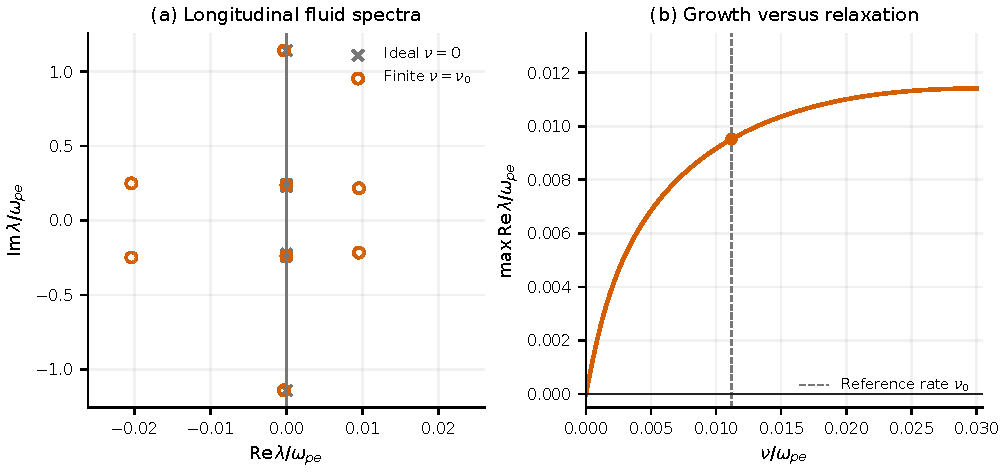
\includegraphics[width=\linewidth]{../figures/stability.pdf}
\caption{Homogeneous longitudinal test with $U/\sigma=1.2$ and
$k\sigma/\omega_{pe}=0.2$. Left: nonzero eigenvalues of the ideal and finite-rate
fluid systems; the static Gauss-constraint mode is excluded. Right: the
largest fluid growth rate as relaxation varies, with
$\nu_0/\omega_{pe}=1/(40\sqrt5)$ marked. The collisionless kinetic reference
has no growing longitudinal electrostatic mode by the Penrose proof above.
This comparison concerns the stated continuum closure, not an observed mode
in the original reconnection calculation.}
\label{fig:stability}
\end{figure}

\section{A secondary continuity clarification}
\label{sec:continuity}
On PDF p.~5, the source attributes its one-fluid density deficit to the
vanishing of $u_y$ at the symmetric mid-plane, describing this as blocking
transport into the sheet~\cite{original}. The value of a flux at one plane
does not determine its divergence:
\begin{equation}
 \partial_t n=-\partial_x(nu_x)-\partial_y(nu_y).
 \label{eq:continuity-law}
\end{equation}
In particular, $\partial_y(nu_y)$ can be nonzero where $u_y=0$.
This is standard continuum kinematics, not a new plasma mechanism. Its role
here is to qualify an explanation based on symmetry alone; the observed
one-fluid density deficit and its dynamical cause remain separate questions.

\begin{proposition}[A periodic density-accumulation example]
\label{prop:stagnation-density}
For $a,n_0>0$, on a periodic coordinate $y\in[0,2\pi)$,
\begin{equation}
 u_y(y)=-a\sin y,\qquad
 n(y,t)=\frac{n_0}{\cosh(at)-\cos y\,\sinh(at)}
 \label{eq:periodic-counterexample}
\end{equation}
is a smooth positive solution of the one-dimensional continuity equation.
Its total mass is $2\pi n_0$, and
$u_y(0)=0$ while $n(0,t)=n_0e^{at}$.
\end{proposition}
\begin{proof}
The denominator is positive for every finite $t$.
Differentiating \eqref{eq:periodic-counterexample} gives
$\partial_tn+\partial_y(nu_y)=0$ directly. The standard integral
$\int_0^{2\pi}(A-B\cos y)^{-1}\dd y=2\pi/(A^2-B^2)^{1/2}$,
with $A=\cosh(at)$ and $B=\sinh(at)$, gives the conserved mass.
Evaluation at zero gives the stated increasing central density.
\end{proof}

This is an exact kinematic transport example, not a self-consistent
plasma--Maxwell solution or a substitute reconnection run. It refutes the
inference from symmetry alone. The two-population model's total density and
density-weighted velocity obey exactly the same continuity equation after
the population equations are summed. A one-fluid model loses the separate
population-crossing information, but it is not geometrically forbidden from
supplying or accumulating total density within a finite-width layer.
Differences in the evolution of aggregate pressure and higher moments can
still explain a particular benchmark failure.

\section{Conditioning a relative heat-flux accuracy claim}
\label{sec:conditioning}
The source's Eqs.~(3)--(4) and (B1)--(B2) are correct. For $n_1,n_2>0$, put
$n=n_1+n_2$, $w_s=n_s/n$, $\Delta u=u_1-u_2$ and
$T_s=p_s/n_s$. Recentring each population on the aggregate mean gives
\begin{align}
 p_{ij}&=p_{1ij}+p_{2ij}+mnw_1w_2\Delta u_i\Delta u_j,\nonumber\\
 q_{ijk}&=q_{1ijk}+q_{2ijk}
 +nw_1w_2\bigl(\Delta u_i\Delta T_{jk}
             +\Delta u_j\Delta T_{ik}+\Delta u_k\Delta T_{ij}\bigr)\nonumber\\
 &\hspace{15mm}
 -mnw_1w_2(w_1-w_2)\Delta u_i\Delta u_j\Delta u_k.
 \label{eq:mixture-correct}
\end{align}
The source explicitly defines the unnormalized three-term symmetrization,
so its tensor formula has the required scalar factor three. Direct positive
finite-mixture calculations, including nonunit mass, verify all entries.

For the scalar $xxx$ component and $\Delta u\ne0$, define
$\theta_s=T_{sxx}/[m(\Delta u)^2]$. Its counter-streaming contribution is
\begin{equation}
 q_{\rm CS}=mn(\Delta u)^3C,\qquad
 C=w_1w_2\{3(\theta_1-\theta_2)-(w_1-w_2)\}.
 \label{eq:dimensionless-cs}
\end{equation}
Thus the source's cubic-drift explanation of the empirical parameter collapse
requires qualification. Equation~\eqref{eq:dimensionless-cs} also contains a
temperature-contrast term linear in drift and can vanish by symmetry or
cancellation.

\begin{proposition}[A sufficient conditioned relative-error bound]
\label{prop:conditioned-relative-bound}
Suppose $|q_{sxxx}|\le mn_s a_s v_{{\rm th},s}^3$, with
$v_{{\rm th},s}=(T_{sxx}/m)^{1/2}$ and stated nonnegative bounds $a_s$. Set
$E=\sum_s w_sa_s(v_{{\rm th},s}/|\Delta u|)^3$.
If $E<|C|$, then
\begin{equation}
 \frac{|q_{xxx}-q_{\rm CS}|}{|q_{xxx}|}
 \le\frac{E}{|C|-E}.
 \label{eq:conditioned-bound}
\end{equation}
\end{proposition}
\begin{proof}
The exact residual is $r=q_{1xxx}+q_{2xxx}$, so
$|r|\le mn|\Delta u|^3E$. The reverse triangle inequality gives
$|q_{xxx}|\ge mn|\Delta u|^3(|C|-E)>0$.
Division gives \eqref{eq:conditioned-bound}.
\end{proof}

The bound is sufficient rather than necessary. Its imbalance/cancellation
factor cannot be dropped. Equal population densities and temperatures give
$q_{\rm CS}=0$ at any drift. With equal densities but unequal temperatures,
$q_{\rm CS}=3n\Delta u\,\Delta T_{xx}/4$, which is linear in drift.

\paragraph{A near-Maxwellian counterexample to a speed-ratio-only guarantee.}
Let $W$ take values $-1/\sqrt2$ and $\sqrt2$ with probabilities $2/3$ and $1/3$.
Then $\E{W}=0$, $\E{W^2}=1$ and $\E{W^3}=1/\sqrt2$.
For $\eta>0$, let $S=(W+\eta G)/\sqrt{1+\eta^2}$ with $G$ a standard Gaussian.
Let $H=(S,G_y,G_z)$, with independent standard Gaussian transverse components,
and define $X_\epsilon$ to have law
$(1-\epsilon)\mathcal N(0,I)+\epsilon\mathcal L(H)$, $0<\epsilon<1$.
It has zero mean, covariance $I$, and third moment
$\E{X_{\epsilon,x}^3}=\epsilon/[\sqrt2(1+\eta^2)^{3/2}]$.
Its total-variation distance from $\mathcal N(0,I)$ is at most $\epsilon$.
Give the populations equal densities and velocity laws
\begin{equation}
 V_1=Ue_x+\sigma X_\epsilon,\qquad
 V_2=-Ue_x+\sigma X_\epsilon.
 \label{eq:smooth-skew-mixtures}
\end{equation}
Each population density is a positive smooth Gaussian mixture, within
$\epsilon$ in total variation of its matching Maxwellian. Their intrinsic
temperature tensors are both $m\sigma^2I$, so
$q_{\rm CS}=0$, whereas
$q_{xxx}=mn\sigma^3\epsilon/[\sqrt2(1+\eta^2)^{3/2}]\ne0$.
Consequently the relative closure error is one even when both $\epsilon$ and
the thermal-to-beam speed ratio $\sigma/U$ are arbitrarily small.
The absolute residual does tend to zero relative to $mnU^3$.
The recorded calculations use $\epsilon=0.01$ and integrate the smooth
laws with positive Gauss--Hermite quadrature.

This construction does not disprove the source's measured collapse in its
particular family of reconnection simulations. It identifies assumptions
needed to extend that empirical observation to a relative-error guarantee.
The source scan uses initial speeds; inserting those into a local bound would
also require estimates of their subsequent evolution.

\paragraph{The valid limitation of a memoryless one-fluid closure.}
Additional population information can be genuinely necessary. For example,
let $n=m=1$, and let each population be an isotropic Gaussian of variance
$3I/4$. Choose a weight $w$, set
$\Delta=[4w(1-w)]^{-1/2}$, and assign means
$(1-w)\Delta e_x$ and $-w\Delta e_x$.
For both $w=1/2$ and $w=1/4$, the aggregate density is one, the mean is zero,
and the pressure is $\diag(1,3/4,3/4)$. The respective $q_{xxx}$ values are
zero and $1/(4\sqrt3)$. Hence no arbitrary-distribution algebraic function
of only $n,u,p$ can recover both third moments. This supports the source's
population-resolving motivation. It is not an impossibility statement for
one-fluid descriptions with memory, extra variables, gradients or nonlocality.

\section{Finite isotropization over a comparison interval}
\label{sec:entropy}
The source openly retains isotropization for numerical stability~\cite{original}.
Its smallness relative to a fast local heat-flux scale does not establish
closeness to zero-intrinsic-heat-flux evolution over an entire simulation.
A homogeneous calculation makes the distinct finite-time parameter explicit.

At fixed density, let $p$ be a positive-definite pressure tensor and
$\bar p=\tr p/3$. The relaxation part alone satisfies
\begin{equation}
 \dot p=-\nu(p-\bar p I),\qquad
 p(t)=\bar p I+e^{-\nu t}\bigl(p(0)-\bar p I\bigr).
 \label{eq:homogeneous-isotropization}
\end{equation}
Its trace, and thus its thermal energy, are constant. For the Gaussian
entropy diagnostic per particle,
$s_G=\tfrac12\log\det p-\tfrac52\log n+\text{constant}$, one obtains
\begin{equation}
 \dot s_G=\frac{\nu}{2}
 \bigl(\bar p\,\tr(p^{-1})-3\bigr)\ge0,
 \label{eq:entropy-production}
\end{equation}
with equality only at isotropy. The inequality follows by applying the
arithmetic--harmonic mean inequality to the three positive eigenvalues of $p$.
This is an entropy diagnostic of the moment model, not a measurement of
PIC entropy or evidence of external heat input.

The deviation from the zero-relaxation homogeneous pressure is controlled by
$1-e^{-\nu T}$, not by $\nu$ alone. At the ideal reference-scale rate
$\nu/\omega_{pe}=1/(40\sqrt5)$ and $T=300\omega_{pe}^{-1}$,
\begin{equation}
 \nu T=3.354101966\ldots,\qquad
 e^{-\nu T}=0.0349407340\ldots.
 \label{eq:finite-relaxation-duration}
\end{equation}
Thus an initially present homogeneous anisotropy would retain about $3.49\%$
of its amplitude over that interval. For the example
$p(0)=\diag(2,1/2,1/2)$ at unit density, the entropy diagnostic increases
by $0.3461208970\ldots$ while the trace remains three.

This example does not establish how much relaxation changes the evolving
source current sheet, whose anisotropy is time-dependent. It shows why a
finite-duration sensitivity study in $\kappa$, or a direct comparison of the
retained pressure-source terms, is needed when interpreting the implementation
as approximately zero-heat-flux evolution. It does not dispute the source's
disclosed need for finite stabilization, nor identify irreversible adiabatic
relaxation with external energy transfer.

\section{Reproducible calculations and evidence limits}
\label{sec:reproducibility}
The repository separates reanalysis of archived simulation output from
analytical model tests. The initial-state analysis uses the authors' data
dictionary, independently readable HDF5 attributes, published input decks,
and explicitly aligned grid locations. The stability, continuity and moment
calculations use specified equations and inputs and require no reconnection
simulation executable.

The inspected Zenodo record is identified by the record-specific DOI
\href{https://doi.org/10.5281/zenodo.21114117}{10.5281/zenodo.21114117};
the source's concept DOI is
\href{https://doi.org/10.5281/zenodo.21114116}{10.5281/zenodo.21114116}.
Both resolve to this dataset family.
The registration agency is DataCite, whose API identifies the record DOI as
findable; a Crossref-only lookup returns no record. The direct repository
link is \url{https://zenodo.org/records/21114117}. These identifiers do not
denote two different simulations or a replacement data source.

\begin{table}[tbp]
\centering
\small
\caption{Selected verification outcomes. The code, data definitions and scope limits distinguish initial-state reanalysis from independent continuum tests.}
\label{tab:verification}
\begin{tabular}{p{.48\linewidth}p{.43\linewidth}}
\toprule
Check & Outcome \\
\midrule
Initial moment current at $Y=16.05d_e$ & 11.5309\% below staggered curl \\
Initial $P_{zz}/p_{\rm fl}$ at that row & 0.615446655 \\
Exact mixture identities & All scalar and tensor checks pass \\
Symmetry-plane continuity & Zero normal velocity; increasing density \\
Conditioned relative-error example & 0.024134 $\le$ 0.036243 \\
Identical one-fluid lower moments & Different third moments \\
Finite-relaxation mode growth & $0.009518499\,\omega_{pe}$ \\
Homogeneous relaxation over $300/\omega_{pe}$ & 3.4941\% anisotropy remains \\
\bottomrule
\end{tabular}
\end{table}


The data retriever requests only selected ZIP members from the public Zenodo
archive. It requires bounded HTTP partial responses, checks member lengths
and CRC32 against the ZIP directory, and records SHA-256 hashes of the
extracted inputs. The published checksum of the complete archive is identified
as publisher-supplied; a partial retrieval does not verify that whole-archive
checksum. Small derived profiles and provenance are included with their
attribution. The original paper and full simulation archives are not
redistributed by this project.

Numerical checks preserve the exact mixture identities rather than treating
them as errors. The linear calculation is checked independently through an
eliminated dielectric relation and the Gauss constraint, in addition to the
matrix eigenvalue residual. The kinetic comparison has an exact rational
stability bound, so its conclusion does not depend on locating a numerical
threshold near marginal stability. The continuity example satisfies the
transport equation explicitly. These checks test the scientific statements
used in the paper, not only whether a plotting script runs.

The execution record in Appendix~\ref{app:execution} pins the code, input
hashes, numerical results and environment. Its timestamps are author-environment
execution evidence, not third-party certification or independent human peer
review. The accompanying verification script reports actual failures instead
of silently replacing absent inputs with synthetic data.

No OSIRIS or Gkeyll reconnection run was performed for this study. The
published input decks and archived diagnostics do not uniquely identify the
authors' exact executable builds. In particular, the documented custom
velocity diagnostics are interpreted using the authors' explicit data
dictionary; we do not assert that a present public source checkout is the
private build that produced them. This limits claims about implementation
internals while leaving the documented archived-moment comparison testable.

\section{Consequences for controlled validation}
\label{sec:discussion}
An initialization audit should precede attributing every later difference to
the heat-flux closure. The current test exposes a mismatch in physical moments
despite matching algebraic drift expressions. A controlled repeat should match
density, ordinary mean velocity and the selected pressure definition, and
report the initial magnetic curl and moment current on their actual staggered
locations. If relativistic particle initialization and a nonrelativistic fluid
model are compared, the conversion and the target moment convention must be
stated explicitly. The cold proper-velocity conversion alone is not a proof
that finite-temperature moments have been matched.

The clean one-fluid endpoint contrast establishes a numerical response to
the aggregate-moment intervention: all four tested endpoint errors decrease.
It does not establish a physical cause of the source's reconnection differences.
The intervention replaces the conserved moment vector through second order,
including sampled spatial variation; it is not confined to the mean current.
Both one-fluid saved histories have covariance
failures, the clean unmatched two-fluid endpoint is rejected, and the matched
two-fluid run fails before producing its comparison endpoint. A smaller
endpoint error cannot erase those failures or substitute for realizability
and resolution checks. We therefore do not infer that correcting the drift
eliminates the reported density deficit, reproduces full PIC heat flux with
one fluid, or reverses the source's physical conclusion.

The archived one- and two-fluid endpoints remain positive definite under
the same tensor test. This distinguishes an observed failure of the identified
clean implementation from a claim about the unavailable dirty executable.
The finite snapshot archive does not establish that the original intermediate
trajectory was admissible, either. Identified executable provenance, full-tensor
state checks and grid-converged controls are needed before transferring the
numerical endpoint changes into a physical causal statement.

The auxiliary homogeneous stability test supplies a separate calibration.
Retaining population drift creates the possibility of streaming modes; it
does not ensure the correct kinetic susceptibility or growth rate. The
implemented relaxation should be included in the dispersion calculation.
Finite relaxation can change a spectrum even when the unperturbed pressure
is isotropic and the relaxation source vanishes at equilibrium. In the stated
example the resulting growing mode is a false positive relative to the
collisionless kinetic reference. This is a test of a model's continuum
response, not evidence that the original simulation visibly contains that mode.
The new clean-source evolutions do not provide a source-sheet eigenanalysis
or a physically validated, grid-converged matched comparison. This diagnostic
comment quantifies numerical sensitivity and exposes validation requirements;
the source's nonlinear physical conclusions are not thereby disproved.

The pressure-source diagnostic should also distinguish a third-moment amplitude
from its divergence. The scale proxy $p\,d_e/|q|$ used in the source is a useful
estimate when $d_e$ is an appropriate gradient length. It is not identical to
$p/|\nabla\!\cdot q|$. A spatially constant nonzero heat-flux tensor has a finite
amplitude proxy and zero divergence. The source explicitly notes that its
isotropization closure constrains a divergence and omits the reconstructed
fluid tensor from some plots; we do not characterize that disclosure as a
hidden omission. Direct source-term comparisons and rate convergence would
make the approximation more informative.

Finally, the source's time-maximum spatial score is a best-time diagnostic,
not a uniform-in-time error bound or a forward prediction test at every scan
point. The conditioned estimate above explains why both absolute residuals
and a nondegenerate denominator are needed when assessing relative accuracy.
These qualifications preserve the observed scan and suggest measurements
needed before extending its interpretation to new current sheets, later
island recirculation, or turbulence.

The valid component-to-aggregate moment decomposition remains the foundation
of this analysis. Additional labels carry information absent from a generic
state described only by total density, velocity and pressure. The corrections
identify controls and assumptions needed for using that additional information
reliably, rather than a general rejection of multicomponent fluid modeling.

\section{Conclusion}
Matching a nominal drift expression does not match a proper-momentum PIC
initialization to an ordinary-velocity fluid initialization. The archived
initial moments make that distinction quantitatively testable.
Resolving two populations also does not ensure faithful kinetic instability
growth: finite isotropization must be validated as part of the closure.
The exact moment decomposition remains valid and useful. Correcting the
density-transport explanation and conditioning relative-error statements
provides a constructive basis for further comparison, without asserting
that the reported nonlinear reconnection results have been disproved.

\section*{Author and methods disclosure}
Taylor Kalin is the author and is responsible for this study. OpenAI Codex
assisted with source inspection, derivations, code, data analysis, and manuscript
preparation under his direction. Separate AI-agent checks were used during
preparation; they are not represented as independent human expert review.
Reported results are deterministic classical computations and reanalysis of
public archived moments. No new reconnection simulation or experimental
measurement is claimed.

\paragraph{Funding and competing interests.}
This study was self-funded by Taylor Kalin, including computing resources and
AI tools. No external funding was received. No competing interests were
reported for this study.

\section*{Prior dissemination and review sequencing}
This is one study. GitHub and AiraXiv deposits are preprint versions of the same
work. Agent-only editions, where used, identify Taylor Kalin as canonical
author and human operator; they are not independent new findings.
Review venues are sequenced to avoid concurrent consideration of the same
manuscript. Actual identifiers and outcomes are recorded at
\url{https://github.com/Teylersf/counterstreaming-heatflux-audit}
in the publication-status record.

\bibliographystyle{unsrt}
\bibliography{references}
\appendix
\section{Source passages and artifact scope}
\label{app:source-evidence}

All source equation and page locators refer to the PDF of
arXiv:2607.07106v1~\cite{original}. The supplied ten-page PDF is byte-identical
to a fresh versioned arXiv download: 7,847,791 bytes, SHA-256
\begin{quote}\footnotesize\ttfamily
fc5344e2ba8f4db98baf90d805bb6b7c\\
e8835c32ea7bf54bba4d62f405b955a3.
\end{quote}
The official history checked on 28 October 2026 lists v1 submitted
8 July 2026 at 07:43:25 UTC, with no later revision or journal reference.
The PDF displays 9 July; the experimental HTML displays 24 August. The original
\texttt{apssamp.tex}, line 95, uses \verb|\date{\today}|, so separately compiled
display dates are not version identifiers. No source author has been contacted,
and no author confirmation is claimed.

The separately retrieved
\href{https://arxiv.org/src/2607.07106v1}{versioned source archive} has
7,439,982 bytes and SHA-256
\begin{quote}\footnotesize\ttfamily
4f9abd5f41ffca0f1879981429165ff1\\
a989276792c812e860f57cb5038c3b2e.
\end{quote}
The repository's
\href{https://github.com/Teylersf/counterstreaming-heatflux-audit/tree/main/source-excerpts}{selective excerpts}
contain six attributed files and 17 fragments, with original TeX line and
character positions. A standalone verifier checks the archive and source
hashes and reconstructs every excerpt without executing the source or making
network requests. The full PDF and source archive are not redistributed.

\paragraph{The stated initialization.}
Appendix A, p.~6, states that the electron fluid velocities are initialized from
\[
 \epsilon_{ijk}\partial_j B_k=J_i=q_e n_0\overline v_i.
\]
Appendix C, p.~8, states that the fluid simulations inherit the PIC domain,
grid, boundary conditions and magnetic-field initial condition exactly. It
specifies the common initial drift
\[
 \overline v_{1i}=\overline v_{2i}=\overline v_i
\]
and thermal speed $0.111803c$ for the electron fluids. These are the
matching statements tested in the main text. Original TeX locators are
lines 225, 244 and 280; the printed seed is Eq.~(A3), lines 238--240.

The current public \texttt{udist} documentation describes \texttt{ufl} and
\texttt{spatial\_ufl} as fluid momentum in proper-velocity units and gives
relativistic momentum addition as the default~\cite{osirisudist}. This documents
the input-language interpretation; it does not identify the authors' exact
historical executable. For the archived diagnostics, the definition used here
comes directly from the authors' Zenodo deposit description~\cite{dataset}:
\[
 \mathrm{vfl}_i=\frac1n\int f v_i\,\dd^3v,
 \qquad
 (v_i v_j)_{\rm diagnostic}=\int f v_i v_j\,\dd^3v.
\]
The deck and diagnostic checks, rather than an assumed private code revision,
support the initial-moment comparison.

\paragraph{The density-transport explanation.}
The main text, p.~5, attributes the one-electron-fluid density deficit to the
following mechanism:
\begin{quote}\small
``at the mid-plane $\overline v_y=0$ by symmetry, blocking 1-e-Fluid transport
into the sheet''.
\end{quote}
The complete argument is in original TeX line 191. The symmetry-plane
continuity calculation assesses this causal explanation; the plotted density
deficit remains empirical evidence from the reported benchmark.

\paragraph{The implemented closure and instability claim.}
On p.~4 the source specifies the finite local model
\[
 \partial_m q_{ijm}=\kappa v_{th}(p_{ij}-\delta_{ij}p),
 \qquad p=\tr(p_{ij})/3,\qquad \kappa=0.1d_e^{-1},
\]
with an isotropization timescale of about $90\omega_{pe}^{-1}$
(original TeX line 179). Figure~3's caption, p.~4, explicitly omits its
contribution from the displayed fluid heat flux and notes that only its
divergence is constrained (line 166). The finite term is therefore a disclosed
part of the model. The longitudinal calculation in this study tests that
finite model, rather than silently replacing it by its zero-coefficient limit.
On p.~5 the source also asserts that the two-electron-fluid model can capture
linear growth because the instabilities are due to counter-streaming
(line 207). The general importance of closure choice for instability fidelity
is established prior context~\cite{ng2019}.

\paragraph{Accuracy metric and retained qualifications.}
The color in source Fig.~4, p.~5, is the best-time score
\[
 \max_t\left[
 1-\frac{\langle|q_{xxx}-q_{CSxxx}|\rangle_{xy}}
 {\langle|q_{xxx}|\rangle_{xy}}
 \right]
\]
(original TeX line 198). Its proposed thermal/drift scaling is explained in
line 202. The present audit distinguishes this empirical best-time diagnostic
from a uniform error guarantee; it does not claim to have rerun the parameter
scan. The source acknowledges later stream folding (p.~5, line 207), separate
fluid color scales and amplitude differences in the full-tensor comparison
(Fig.~5, p.~7, line 250), and kinetic free-expansion limitations
(Appendix C, p.~8, line 293). The exact mixture identities in source
Eqs.~(3)--(4) and (B1)--(B2) are preserved as valid algebra.

\section{Pinned execution record}
\label{app:execution}
The reported calculations use the immutable code commit:
\begin{quote}\small
\href{https://github.com/Teylersf/counterstreaming-heatflux-audit/tree/e1ebd1aaee17bc5cd486d40387eb655aefd70c20}{\texttt{e1ebd1aaee17bc5cd486d40387eb655aefd70c20}}
\end{quote}
This pins the numerical code and inputs; the final release also contains the manuscript source.
\begin{verbatim}
git clone https://github.com/Teylersf/counterstreaming-heatflux-audit.git
cd counterstreaming-heatflux-audit
git checkout e1ebd1aaee17bc5cd486d40387eb655aefd70c20
python -m pip install -r requirements.txt
python experiments/fetch_data.py
python experiments/data_checks.py
python -X utf8 experiments/verify.py
python -X utf8 experiments/make_figures.py
\end{verbatim}
This is an author-environment execution record, not third-party certification or independent human peer review.
\begin{verbatim}
Started UTC: 2026-10-28T23:09:06.987425+00:00
Python: 3.12.14 (main, Aug 25 2026, 14:01:42) [MSC v.1944 64 bit (AMD64)]
NumPy: 2.3.5
h5py: 3.16.0
PASS: initial_current
PASS: initial_pressure
PASS: mixture_identities
PASS: continuity_symmetry
PASS: conditioning_counterexample
PASS: singlefluid_nonidentifiability
PASS: finite_relaxation_stability
PASS: isotropization_entropy
All assertions passed: true
Exit status: 0
\end{verbatim}
\begin{center}
\scriptsize
\begin{tabular}{@{}p{.34\linewidth}p{.63\linewidth}@{}}
\toprule
File & SHA-256 \\
\midrule
\texttt{results/verification.json} & \texttt{6e724e564d4ca23bf718d4add4eded9311aa6ebbeb161c4abc606ec750f01491} \\
\texttt{experiments/verify.py} & \texttt{23c64243de9e58d493fc87b18b4c47edf917fb67d11853898009e6e8824903e6} \\
\texttt{experiments/closure\_checks.py} & \texttt{797fa1a2c85b36e09531fcff343ebed773674ecfe5a1caf8bd6518826ed3efbb} \\
\texttt{experiments/data\_checks.py} & \texttt{fb2253e5f1970e80baea7a5349a8ac0cbf0e847b0cfe3f04eadb99b1e32e064b} \\
\texttt{experiments/fetch\_data.py} & \texttt{9739bc225cda81134c984edb9c06a39a36a5c24403d6b67564e6de2d063a6fc0} \\
\bottomrule
\end{tabular}
\end{center}
The full log, input provenance, derived profiles and strict verification JSON are included in the repository.

\end{document}
